\documentclass[a4paper]{jpconf}
\usepackage{graphicx}
\usepackage{lipsum}
\usepackage{minted}
% \usepackage{listings}
\usepackage{parcolumns}
\usepackage[compatibility=false]{caption}
\usepackage{lscape}
\usepackage{pdflscape}
\usepackage{rotating}

\begin{document}
\def\code#1{\texttt{#1}}
\title{Giving \textit{pandas} ROOT to chew on: experiences with the XENON1T Dark Matter experiment}

\author{D Remenska$^{1}$, C Tunnell$^{2}$, J Aalbers$^{2}$, S Verhoeven$^{1}$, J Maassen$^{1}$, \newline J Templon$^{2}$}
\address{$^{1}$Netherlands eScience Center, Science Park 140, Amsterdam, The 
Netherlands}
\address{$^{2}$National Institute for Subatomic Physics (NIKHEF), Science 
Park 
105, Amsterdam, The Netherlands}
\ead{d.remenska@esciencecenter.nl}

\begin{abstract}
In preparation for the XENON1T Dark Matter data acquisition, 
we have prototyped and implemented a new computing model. 
The XENON signal and data processing software is developed fully in Python 3, and makes extensive use of generic scientific data analysis libraries, such as the SciPy stack.
A certain tension between modern ``Big Data'' solutions and 
existing HEP frameworks is typically experienced in smaller particle physics experiments.
ROOT is still the ``standard'' data format in our field, defined by large experiments (ATLAS, CMS).
To ease the transition, our computing model caters to both analysis paradigms, leaving the choice of using ROOT-specific \texttt{C++} libraries, 
or alternatively, Python and its data analytics tools, for developing physics algorithms. 
We present our path on harmonizing these two ecosystems, which allowed us to use off-the-shelf software libraries
(e.g., NumPy, SciPy, scikit-learn, matplotlib) and lower the cost of development and maintenance. 
To analyse the data, our software allows researchers to easily create ``mini-trees'';
small, tabular ROOT structures for Python analysis, which can be read directly into \textit{pandas}
DataFrame structures. One of our goals was making ROOT available as a cross-platform binary for an easy
installation from the Anaconda Cloud (without going through the ``dependency hell'').
In addition to helping us discover dark matter interactions, lowering this barrier helps shift particle physics
toward non-domain-specific code.

% All articles {\it must} contain an abstract. This document describes the  
% preparation of a conference paper to be published in \jpcs\ using \LaTeXe\ and 
% the \cls\ class file. The abstract text should be formatted using 10 point font 
% and indented 25 mm from the left margin. Leave 10 mm space after the abstract 
% before you begin the main text of your article. The text of your article should 
% start on the same page as the abstract. The abstract follows the addresses and 
% should give readers concise information about the content of the article and 
% indicate the main results obtained and conclusions drawn. As the abstract is 
% not 
% part of the text it should be complete in itself; no table numbers, figure 
% numbers, references or displayed mathematical expressions should be included. 
% It 
% should be suitable for direct inclusion in abstracting services and should not 
% normally exceed 200 words. The abstract should generally be restricted to a 
% single paragraph. Since contemporary information-retrieval systems rely heavily 
% on the content of titles and abstracts to identify relevant articles in 
% literature searches, great care should be taken in constructing both.
\end{abstract}

\section{Introduction}

With the recent inauguration of the new XENON1T instrument at the Gran Sasso National Laboratory,
the most sensitive dark matter experiment in the world will boost-up the hunt for this rare-signature particle.
In preparation for the data acquisition, a new computing model has been designed and implemented, making a paradigm
shift from the typical HEP-specific frameworks and tools. 
Python has received a widespread adoption among the scientific community, due to its ease of use for fast prototyping, and
the rich ecosystem of scientific data analysis packages (Numpy, SciPy, pandas, and matplotlib, to name but a few).
Our quick experiment progress gives us more in common 
with a tech startup than most other experiments, which is why we explored community-supported Big Data solutions.
Large HEP experiments have an investment in software spanning 20 years, and mostly use the ROOT framework and data format. 

To ease the tension between these ``novel'' Big Data solutions and the ones typically used in HEP communities,
we interfaced Python \textit{pandas} to ROOT, effectively 
harmonizing these two software jungles, which allowed us to use existing software libraries and leverage our Python experience, while 
leaving the choice of using ROOT-specific \texttt{C++} libraries as an alternative.
PhD students and researchers should not have to spend too much time getting software tools and libraries to work in their own local environment; they 
should rather focus on the physics research. For this, 
we built cross-platform binary ROOT packages that can be easily installed in user space, taking care of all library dependencies.
In this paper we report the technical choices we made in order to meet these challenges, and the resulting impact on the XENON (and wider) community.

\section{The XENON Dark Matter experiment}
Most matter in our Universe is ``dark matter'', yet it remains invisible to our instruments. What
constitutes dark matter is one of the most intriguing questions in modern physics. 
The XENON dark matter experiment~\cite{Aprile2012573},
installed underground at the Laboratori Nazionali del Gran Sasso (LNGS),
aims to detect dark matter in the form interactions of Weakly 
Interacting Massive Particles (WIMPs) with xenon nuclei.
The XENON100~\cite{aprile2014analysis} detector uses a total of 161 kg of 
pure liquid xenon (LXe) divided in cylindrical two-phase  (gas/liquid)  time  projection  chambers.
Its successor, the XENON1T detector~\cite{aprile2013xenon1t}, recently deployed at LNGS, is 
realized by scaling up the existing XENON100 detector by a factor of 10 and reducing the background by a 
factor of 100. With the detector being able to distinguish between the WIMP and possible 
background radiation, the researchers hope to be able to determine the existence of a new subatomic 
particle, and determine its mass and likelihood of interaction with ordinary matter.

\subsection{Computing model and data flow}
In preparation for the XENON1T data acquisition, a new computing model is envisaged. 
The technology chain behind it, is shown on Figure~\ref{fig:XENON1T_flow}.
The experiment data flow contains three parts: acquisition, processing, and analysis. 
The data acquisition system (DAQ), in proximity to the detector, acquires data at a rate of up to 2.4 Gbps, digitizes the PMT signals
and transfers the digitized waveforms from the FADCs (Fast/Flash Analog-to-Digital Converters)
to a local MongoDB storage. The acquisition stage produces cumulatively 1PB of raw BSON-based data
files (binary serialization format) that must be saved to tape.
\begin{figure}[!b]
 \centering
\begin{center}
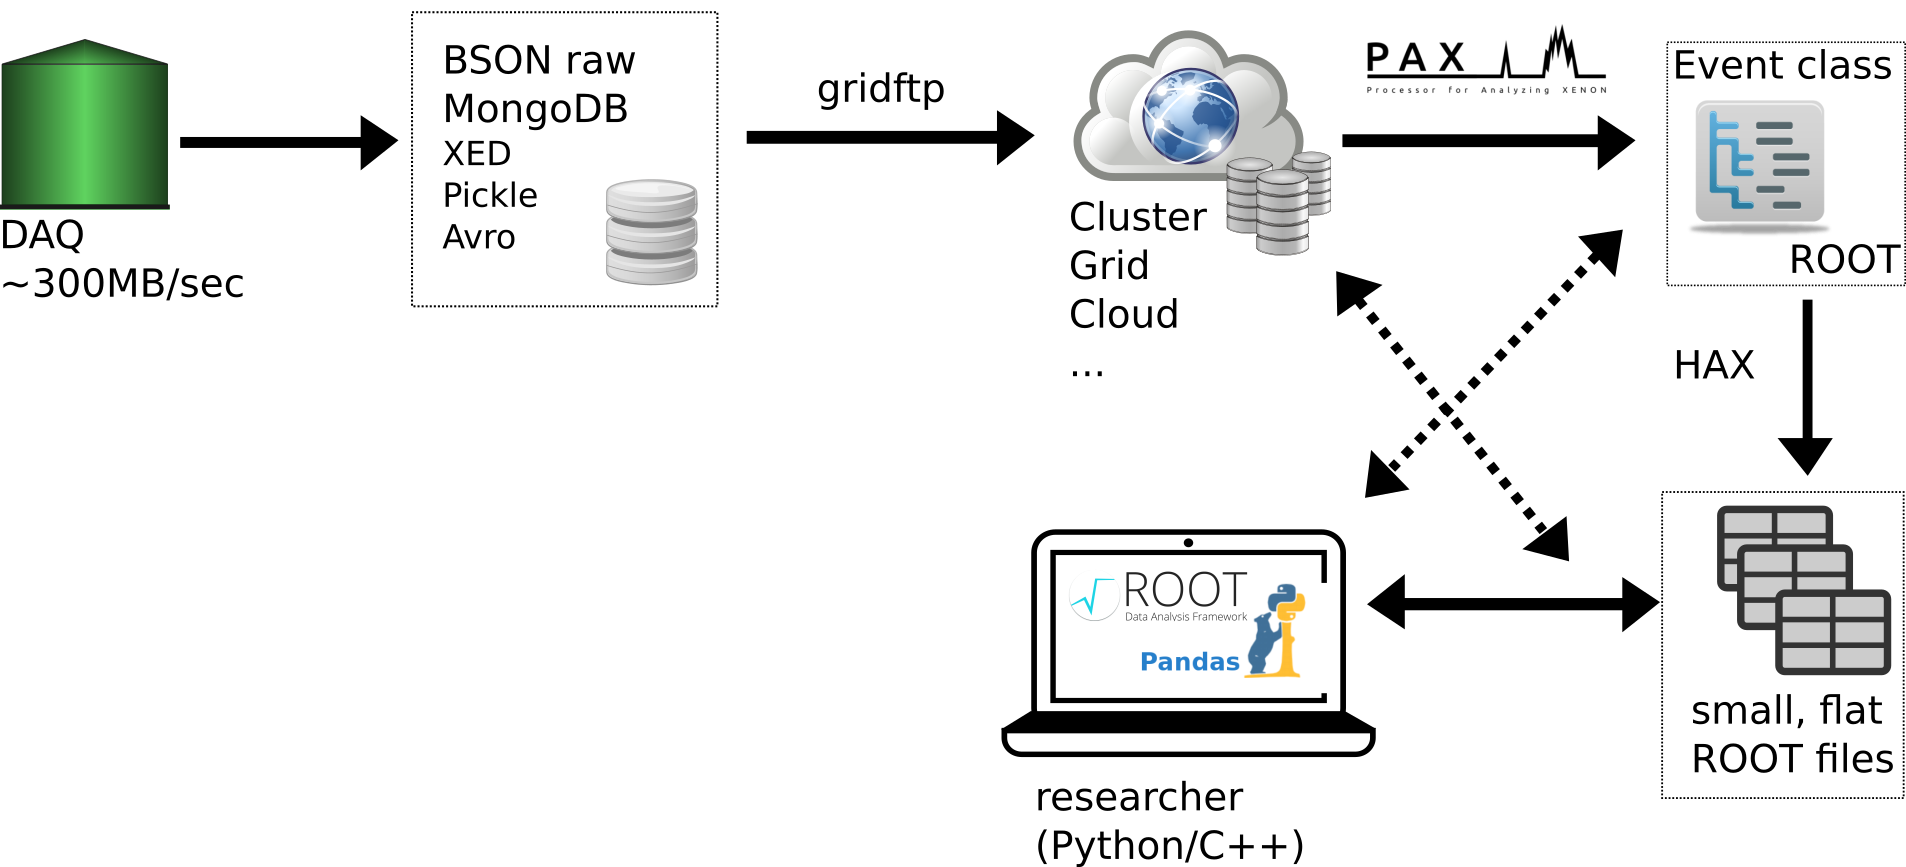
\includegraphics[width=0.8\linewidth]{./graphics/XENON1T_flow1.png}
\caption{XENON1T computing technology chain and data flow}
\label{fig:XENON1T_flow}
\end{center}
\end{figure}
The raw data is subsequently partially processed and reduced using highly optimized trigger routines.
The Celery distributed task queue~\cite{solem2014celery} is used for parallelization. 
%TODO Chris: something about the network upgrade/Tristan?
%TODO Chris something about the previous computing model? C++ vs Python?
At the end of
acquisition, all of the raw data remains within a database at the LNGS site. The utilization of a cloud or grid infrastructure is foreseen in the future, for more efficient larger-scale processing.
The Processor for Analyzing XENON (PAX, Fig.~\ref{fig:paxer}), developed fully in Python 3, is used for digital signal processing and other data processing on the XENON100/XENON1T raw data.
% This program is its own R\&D in both measurement techniques and sustainable
% software development in the sciences.
With a series of I/O and transformation plugins developed for intermediate processing steps, PAX reduces a single event from roughly 1MB
of raw data to 50 KB of processed data. 

The default PAX output format is a ROOT file containing the Event class. 
The processing stage will produce 50 TB of ROOT files, which the analysts must be able to process in an efficient manner. 
For this purpose, the Handy Analysis for XENON (HAX) software was prototyped in Python 3, which 
allows easier and flexible ``pythonic'' access to the ROOT data, without the inconvenience of manually re-looping over the events in one or more ROOT files, each time 
a new plot needs to be created or adjusted. To extract and further reduce the data (make cuts), HAX lets researchers create ``mini-trees'': small, tabular ROOT structures for 
Python analysis that can be read directly into \textit{pandas} DataFrame structures. The main advantage of using them is the easiness of computing over values which 
are not directly in the ROOT tree, compared to the usual \texttt{TTree.Draw} method of analysis where access to the actual values of the data is not directly possible.
In the following section we explain in more details how we implemented this computing model.

\begin{figure}[!t]
 \centering
\begin{center}
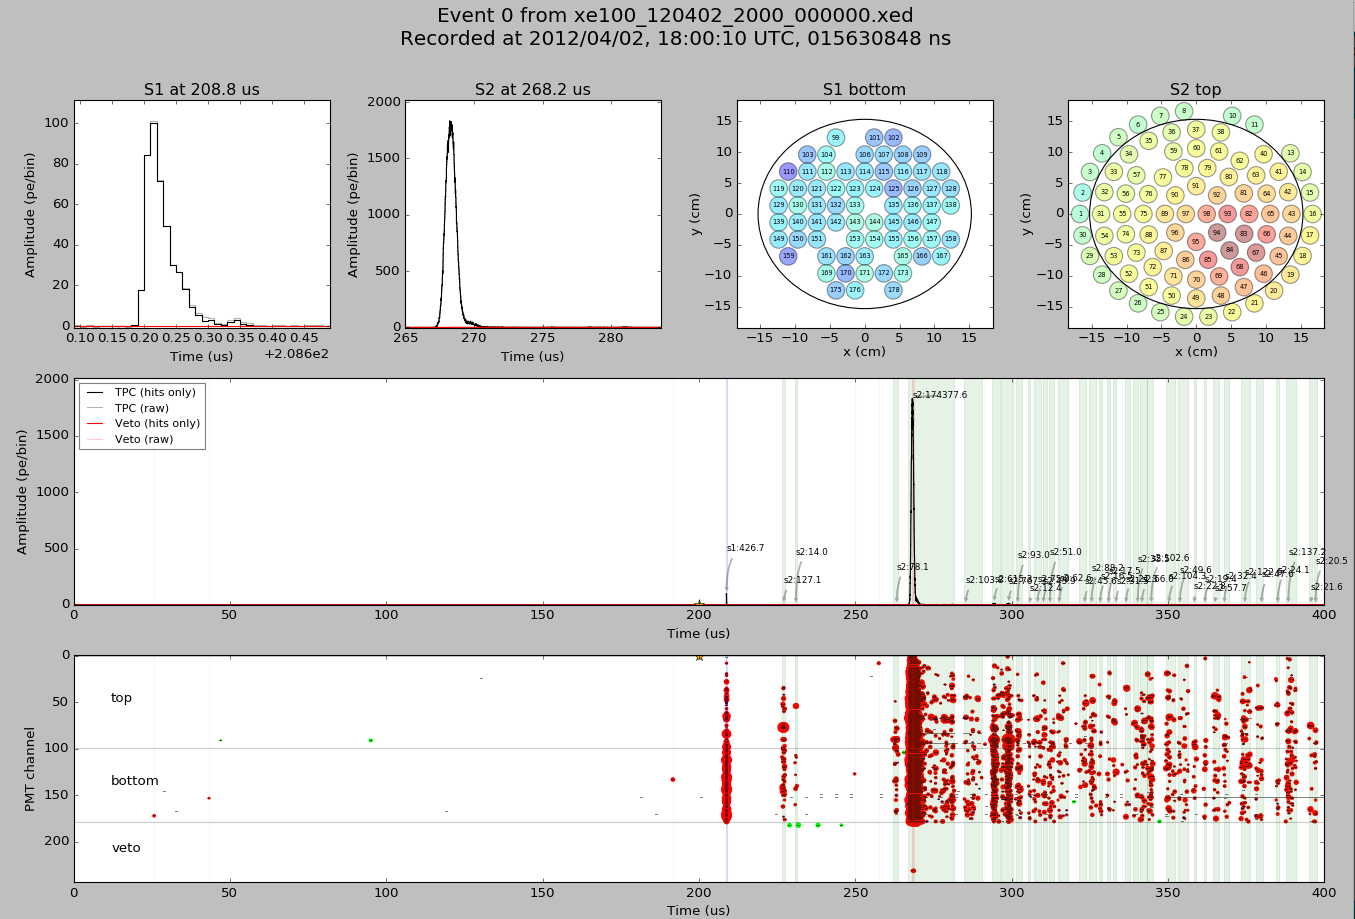
\includegraphics[width=0.9\linewidth]{./graphics/paxer.png}
\end{center}
\caption{Screenshot from the Processor for Analyzing XENON (PAX) software for raw data processing}
\label{fig:paxer}
\end{figure}

\section{Beyond HEP-specific tools}

\begin{figure}[!t]
\centering
\begin{center}
\includegraphics[width=0.65\linewidth]{./graphics/eccosystems1.png}
\caption{Data flows in Particle Physics and Big Data. Interfacing ROOT I/O in Python \textit{pandas} will transitively allow interoperability between existing tools in the two ecosystems}
\label{fig:two_eccosystems}
\end{center}
\end{figure}
The XENON scientific community consists of about 150 researchers, with no dedicated software-expertise manpower. 
The new computing model was prototyped to address some of the issues that small-to-medium-sized particle physics 
experiments face: limited resources and manpower to develop, maintain, and support the necessary software libraries.
The bigger LHC experiments, such as ATLAS and CMS, define the standards of particle physics computing for more than two decades, relying
heavily on CERN's ROOT framework and file format for physics analysis. 
The observation that the HEP computing community is becoming less isolated, is already reported~\cite{1742-6596-513-5-052033}.
However, the process is rather slow, as the HEP community seems to be neither very interested nor ready to accept more mainstream generic solutions, or provide such solutions.
There are exceptions to this, of course, but the list is rather short. 
Examples of projects with beyond-HEP applicability and impact are DIRAC~\cite{1742-6596-119-6-062048}, GEANT4~\cite{agostinelli2003geant4}, and PanDA~\cite{Borodin:1670021}.

On the other hand, generic Big Data analytics tools are gaining a momentum in scientific data analysis, due to the (much) larger and dedicated community support behind these mature tools.
Python has become the language of choice for high-level applications where fast 
prototyping and efficient development are important, while glueing together 
low-level libraries for performance-critical tasks.
The processing software (including the Event data model) is developed fully in Python 3. 
We have found that ensuring correctness via unit testing, integration testing, documentation, and code
sharing in Python and IPython notebooks has many advantages compared to our existing particle
physics codes. We put significant efforts into following Open Source standards and procedures necessary to maintain 
coherent, sustainable, and easy-to-use software. In addition, relying on existing analytics code, instead of particle-physics specific code, greatly
simplifies our work and allows us to focus on the physics.

However, within the XENON collaboration, there is a tension between these ``novel'' Big Data solutions, and the existing ones used in the wider HEP community.
To ease the transition, our computing model should cater to both analysis paradigms, leaving the choice of using ROOT-specific C\texttt{++} libraries, or alternatively, 
Python and its data analytics tools, as front-end framework for developing physics algorithms. 
Hence, our goal is to harmonize these two ecosystems, shown on Fig~\ref{fig:two_eccosystems}, by organizing software and data
such that we can work with the existing particle physics infrastructure, yet still use community Big Data tools.
Specifically, we interfaced Python \textit{pandas} DataFrames to the ROOT format, which allows us to use 
existing software libraries (e.g., NumPy, SciPy, scikit-learn, matplotlib) and lower the cost of developing and maintaining the XENON software stack. 
With pandas I/O to ROOT, we
can also take advantage of tools such as the \textit{odo} project~\cite{odo-pydata} for data migration between storage systems (part of the PyData stack), and allow for conversions between
pandas, HDF5, and MongoDB formats. 
In addition to helping us discover dark matter interactions, lowering this barrier helps shift particle physics
toward non-domain-specific codes.


\subsection{Interfacing ROOT to Python \textit{pandas} DataFrames}
Besides the ``social'' reasons (hesitance to make a big radical leap) for keeping ROOT as the backend file format, 
there are valid technical ones as well: column stores (efficient column scans), continuously improved techniques for pre-fetching, caching, and flushing of data buffers.
Over the past years, the ROOT I/O team has significantly enhanced the I/O performance of ROOT~\cite{1742-6596-331-4-042005}.
However, as already stated, nowadays many ``physics-specific'' analysis algorithms are not that ``physics-specific'' in fact. 
Python has tools and libraries for efficient data structures and array manipulations, with a steeper learning curve than the ROOT analysis framework.
We further elaborate on the existing layers (Fig.~\ref{fig:rootpy_layers}) we used and adapted to fulfill the goal of interfacing ROOT to the Python pandas DataFrames.


\begin{figure}[!t]
\centering
\begin{center}
\includegraphics[width=0.35\linewidth]{./graphics/layers1.png}
\caption{Interfacing ROOT to Python pandas DataFrames. Arrows represent usage dependency.}
\label{fig:rootpy_layers}
\end{center}
\end{figure}

The PyROOT~\cite{1742-6596-664-6-062029} module is a bridge between Python and C. Despite its ROOT bindings,
it is merely a mechanical translation of C\texttt{++} function calls, and as such, programming is not really ``pythonic'', i.e., one 
can not fully leverage existing experience with Python;
the native Python data structures are not used as expected, and these function calls do not adhere to the common Python idioms. 
Furthermore, Python 3 is not yet fully supported, and at the moment of writing, there is no official maintainer of PyROOT.
Often both Python 2 and 3 versions are available on users' systems. However, the official binary releases of ROOT have the PyROOT module built with only Python 2 
support, so PAX users must resort to compiling ROOT from source. Steering the compilation process to look for the correct Python executable and libraries is cumbersome,
and requires setting up environment variables and symlinks. One of our goals was to significantly simplify this process for the collaboration.
In Section~\ref{sec:ROOT_Anaconda} we elaborate our approach to achieving this goal.
In addition, there were blocking Python 3 issues with memory leaks~\cite{JIRA-ROOT-7854} when using array fields, which we had to resolve by patching PyROOT.


\begin{figure}[!h]
 \begin{minipage}{0.5\textwidth}
  \centering
  \begin{minted}[baselinestretch=0.9, fontsize=\footnotesize]{python}
 from rootpy.tree import Tree, TreeModel
 from rootpy.tree import FloatCol, IntCol
 from rootpy.tree import FloatArrayCol, CharCol
 from rootpy.io import root_open
 from random import gauss, choice

 f = root_open("test.root", "recreate")
 # define the model
 class Event(TreeModel):
     s = CharCol()
     x = FloatCol(default = 'nan')
     y = IntCol(default = 0)
     f = FloatArrayCol(5)
 tree = Tree("test", model=Event)
 # fill the tree
 for i in range(5):
     tree.s = ord(choice(ascii_letters))
     tree.x = gauss(.5, 1.)
     tree.y = i
     for j in range(5):
         tree.f[j] = gauss(-2, 5)
     tree.fill()
 tree.write()
 f.close()
  \end{minted}
  \captionof{listing}{Creating tree models with rootpy}
  \label{lst:First_code}
 \end{minipage}
 \begin{minipage}{0.5\textwidth}
  \centering
  \begin{minted}[baselinestretch=0.9, fontsize=\footnotesize]{python}
class ReconstructedPosition(object):
    x = float('nan') 
    y = float('nan') 
    ....

class Peak(object):
    area = 0.0
    detector = 'ptc'
    ...
    rec_positions = list(ReconstructedPosition)

class Hit(object):
    channel = 0
    center = 0.0
    ...
class Event(object):
    event_number = 0
    dataset_name = 'Unknown'
    ...
    peaks = list(Peak)
    hits = np.array([], dtype=Hit.get_dtype())

    \end{minted}
  \captionof{listing}{The pax Event model}
  \label{lst:Second_code}
 \end{minipage}
  \label{lst:representation_examples}
\end{figure}

The rootpy~\cite{noel-dawe-2015-18815} project is a community-driven effort aiming to bring ROOT
closer to the Python arena, on top of the existing PyROOT bindings. In addition to its main capability 
of creating ROOT tree data models purely in Python (Listing~\ref{lst:First_code}) and easier navigation through ROOT files, rootpy provides an 
interface with matplotlib, a popular Python publication-quality plotting library. It can further redirect ROOT error messages through
Python's logging system, turning them into Python exceptions. The related root\_numpy~\cite{noel-dawe-2015-31192}
library is used for efficient conversions between ROOT TTrees and structured NumPy arrays. One can then
take advantage of the statistical and numerical packages that Python offers.
The root\_pandas~\cite{igor-babuschkin-2016-45464} package is a convenience wrapper built around the root\_numpy library. 
It allows to easily load and store pandas DataFrames in the ROOT format.

One essential problem that we stumbled upon, with both rootpy and root\_pandas, is that creating trees with branches 
of user-defined types (and arrays/lists thereof) still requires the necessary ``glue''  C\texttt{++} code. 
We currently autogenerate the C\texttt{++} classes inheriting from TObject, based on introspection of our existing Python Event data model (sketched in Listing~\ref{lst:Second_code}).
Without it, these tools cannot handle nested (json-like) structures, such as the ones PAX uses.
Storing non-rectangular data into Python DataFrames is possible, but it results in object structures that are not easily queried in a manner that flat data 
can be. This is why we created another layer, the HAX analysis tool, which essentially uses root\_numpy under the hood, to load extracted ROOT ``mini-trees'' data into pandas DataFrames.
We were not able to find a suitable mature library or a file format that deals with this type of ``ragged'' data in a more elegant and flexible manner for users.


\section{ROOT in the Anaconda Cloud}
\label{sec:ROOT_Anaconda}

The XENON data processing software makes extensive use of scientific data analysis libraries (such as the SciPy stack).
To make it straightforward for the collaboration users to install the software in user space,
we strongly recommend the Open Source Anaconda Python distribution~\cite{Anaconda_distribution}, which includes many Python scientific modules
bundled in a single installation. This distribution installs all the dependencies cleanly in a single directory (known as \textit{environment}),
and does not interfere with other Python installations present on a system. 
Anaconda comes with a binary packaging, dependency, and environment management system named Conda~\cite{conda}.
It is the main interface for managing multiple installations of various binary packages in separate environments.
Conda environments are not Python-specific, and offer additional advantages compared to virtualenv or pip. 
We aimed to make it easy to re-create consistent environments and be able to reproduce the work of collaboration members, so we adopted Anaconda as a long-term solution in our workflow.

%TODO for introduction, change ``easy'' with convenient or straightforward
As already mentioned, one of the bigger barriers users typically faced was getting ROOT installed in user space. Rather 
than relying on users compiling it with the specific Python 3 bindings and resolving all dependencies themselves,
our goal was to provide a ROOT binary distribution that would be as easy to install as \texttt{conda install root=\{version\}}.
Building a cross-platform binary conda package involves creating a \textit{recipe}, containing metadata on the source code, the build and run dependencies, as well as the scripts 
needed to build the package. In many cases creating a recipe is straightforward; however, making a ``as portable as possible'' ROOT installation is somewhat involved,
due to its dynamic dependencies on \texttt{GCC} and libstdc\texttt{++}.

Linux distributions typically ship a particular version of \texttt{GCC} and \texttt{glibc}.
Our XENON users need to be able to install and run ROOT on a variety of OS versions, ranging from reasonably old to new.
Given that ROOT 6 requires \texttt{GCC>=4.8} to use some of the latest \texttt{C++} features, while we aimed to create a single binary distribution that would work 
out-of-the-box on older systems, we decided to ship \texttt{GCC 4.8} as a ROOT runtime dependency package in conda.
To maintain the ABI (binary) compatibility, and go ``as low as possible'' with \texttt{glibc}, the solution we found is a hybrid one: 
provide a \texttt{GCC 4.8} conda binary that is compiled against an older Linux kernel.
To meet this challenge, Scientific Linux 6 offers a good compromise: the Developer Toolset (v2) from CERN provides 
a newer complier and binutils, while the kernel remains untouched (\texttt{glibc 2.12}). This way we can provide a \texttt{GCC/libstdc++}
that supports the latest \texttt{C++} features, but is still compatible with the oldest \texttt{libc} and kernel we can support.
These technical choices allowed us to produce ROOT (version 5 and 6) conda binaries which have been successfully tested on Ubuntu (11.10, 12.04, 14.04, 15.04) and SLC (6.5 and 7).
The ROOT binaries (with Python bindings for 2.7 and 3.4) and dependencies are available from the Anaconda Cloud, a service for hosting (free public) conda packages.
This also allowed us to do automated integration testing of the XENON data processing software within the Travis CI.
All recipes are also publicly available~\cite{daniela_remenska_2016_47512}, along with a documentation on their usage.

\subsection{Continuous integration}
\begin{figure}[!b]
\begin{center}
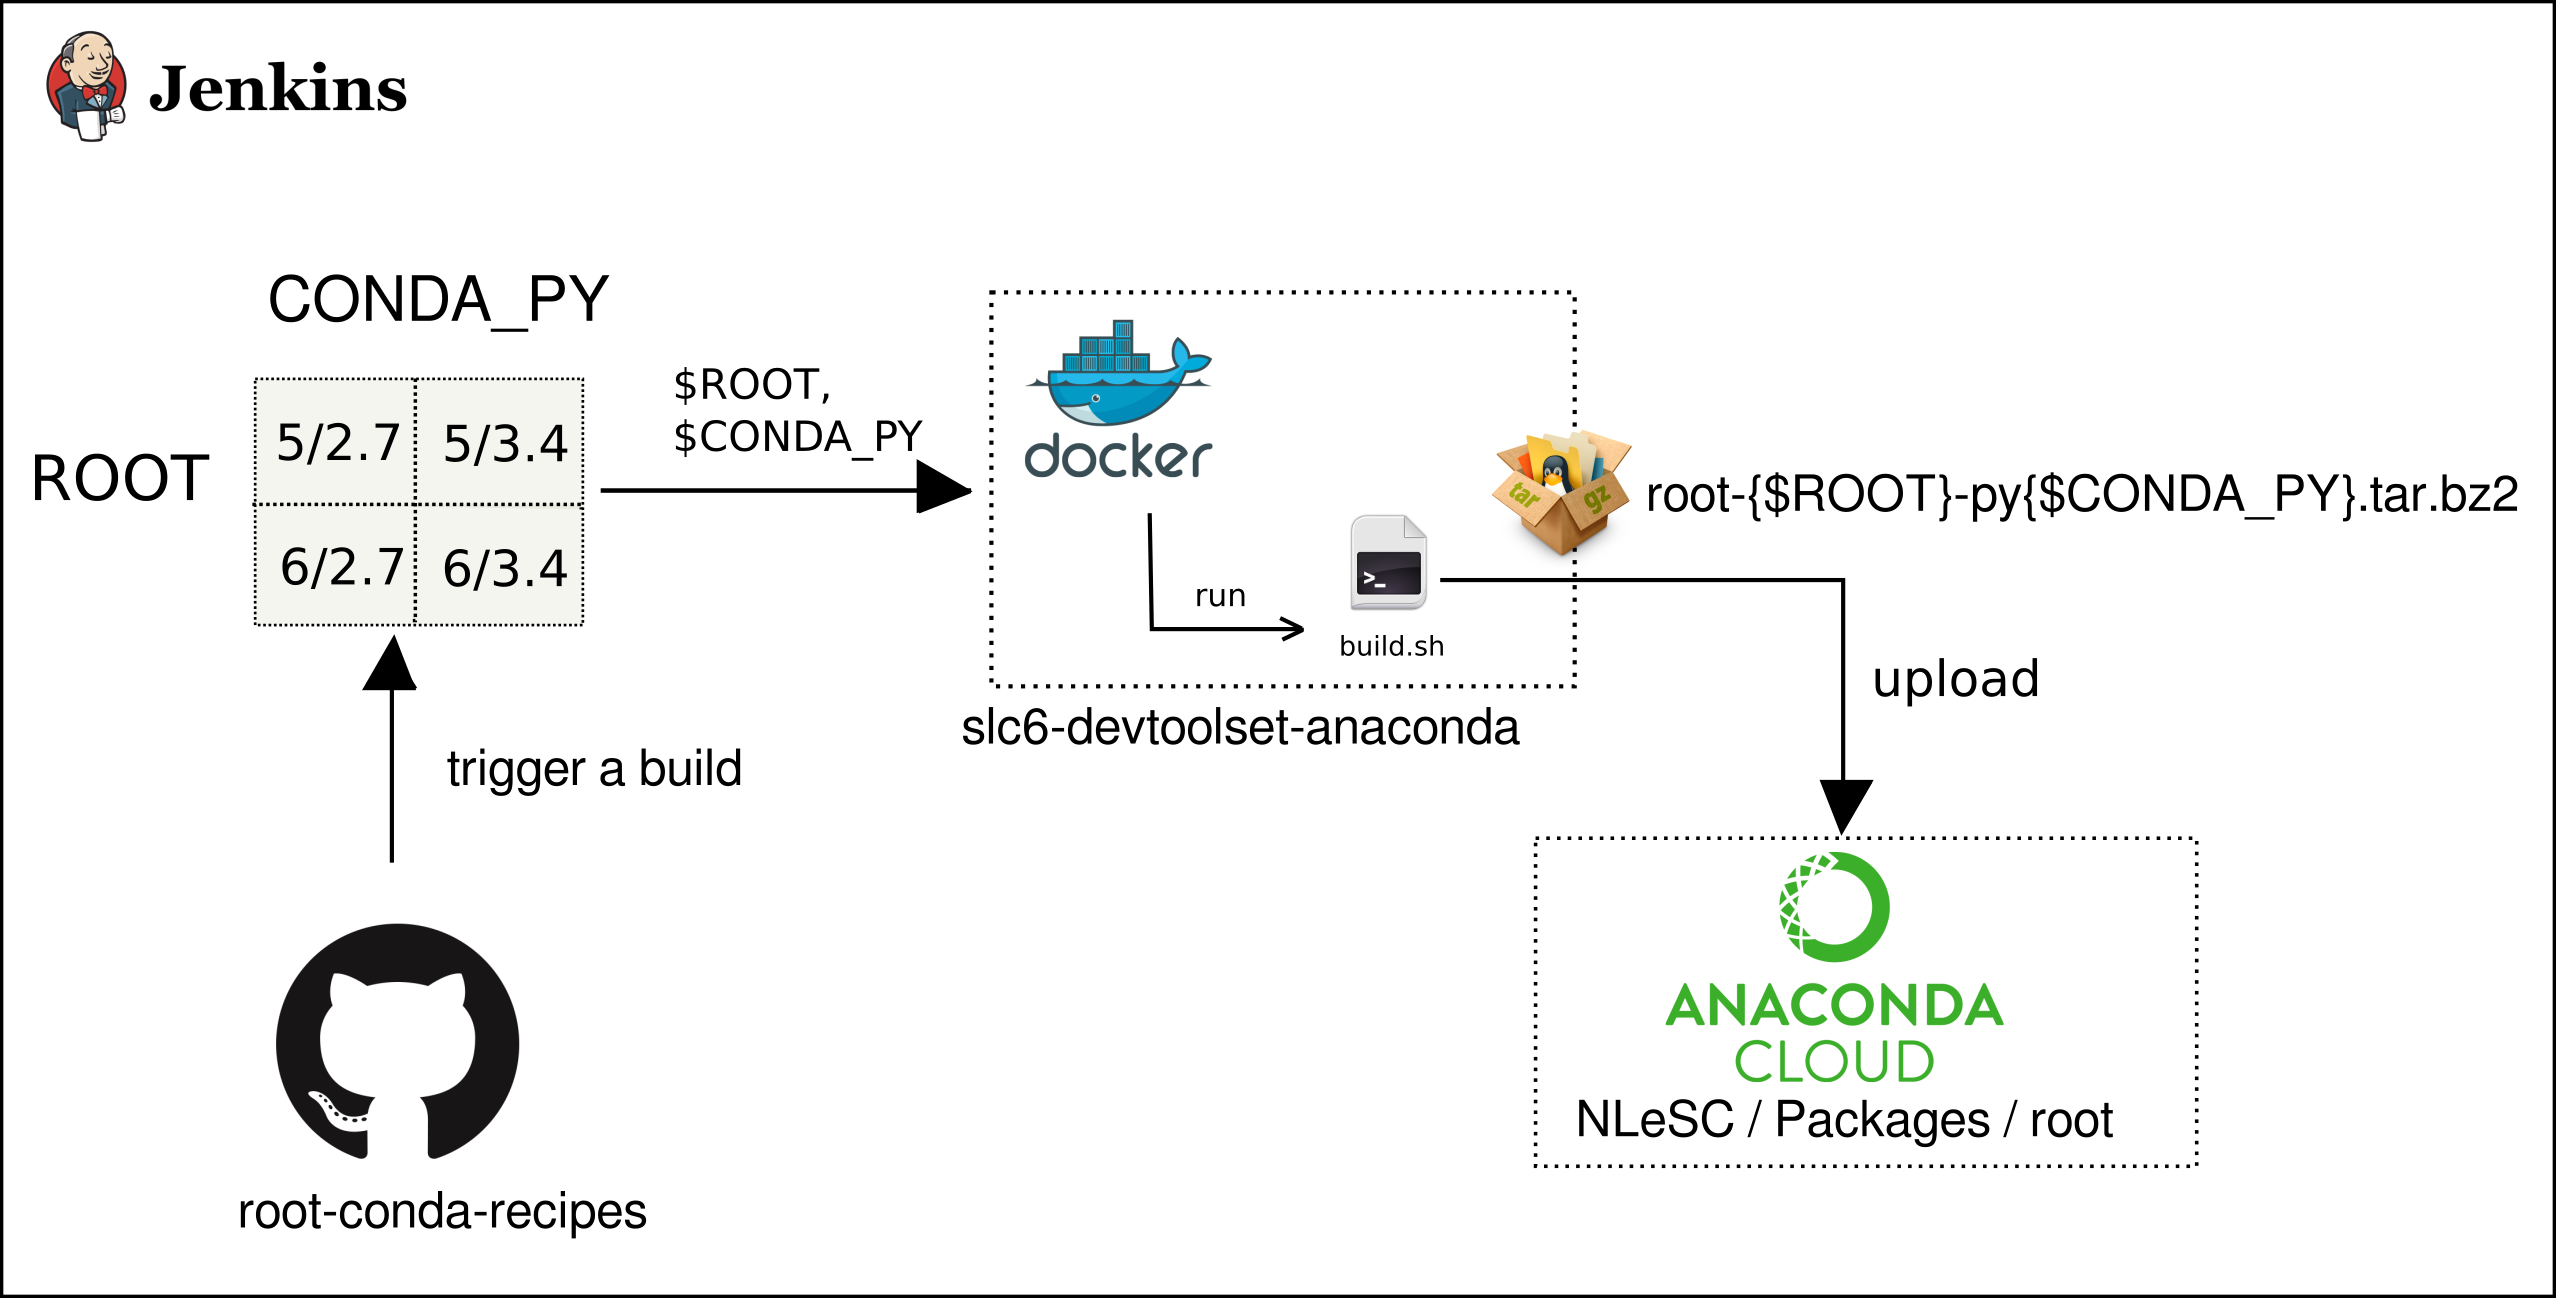
\includegraphics[width=0.8\linewidth]{./graphics/Jenkinssetup2.png}
\caption{Jenkins CI setup for building ROOT binaries and uploading them to Anaconda Cloud}
\label{fig:jenkins}
\end{center}
\end{figure}
Our goal was to have the ROOT (and dependencies) conda packages be automatically rebuilt, tested and uploaded 
to the Anaconda Cloud, triggered by pushing changes to the GitHub recipes repository (for instance, when a new version of the ROOT source code is released). 
There are two mature options for this: Travis and Jenkins CI. 
Travis CI is the most convenient way to automate the builds for both Linux and 
OSX platforms, and it is well integrated as a free service with GitHub. Unfortunately, the current build time restrictions do not 
allow us to build ROOT. Depending on the number of features which are enabled, building and uploading ROOT 6 binaries
 can take up to (more than) 120 minutes, even with 
the most bare-bones configuration.

A public Travis CI setup is used for testing the sanity of existing ROOT conda binaries. 
Once the build-time restriction is lifted or relaxed, switching the building process on, is rather trivial.
For the moment, we rely on an externally-hosted Jenkins machine where we have more resources.
The setup is shown in Fig.~\ref{fig:jenkins}. 
This Jenkins server runs an Ubuntu distribution (12.04, \texttt{glibc 2.15}), where \texttt{GCC 4.8} is not available.
Docker is a container technology that allows for packaging software with all of its dependencies into one image (``lightweight VM''), 
with a guarantee that it will always run exactly the same, regardless of the host environment it is deployed in.
We use it to ship the full build environment for ROOT\footnote{Running a Docker engine requires admin priviledges, which is why we did not use it to provide ROOT binaries directly}.
Each packaged binary of the build-matrix is created using a publicly available Docker image of SLC 6.5, equipped with CERN's Developer Toolset 
(v2), cmake, and conda/Anaconda installed.
\code{CONDA\_PY} and \code{ROOT} are environment variables 
(configurable in Jenkins), and are passed to the \textit{build.sh} script, which contains the \code{conda build} and \code{upload}
commands. Each commit to the \texttt{root-conda-recipes} repository triggers a new build, and the responsible committer will 
receive an email in case of a build failure.

\section{Evaluation}
...some XENON1T workshop trainings?
Jeff's anaconda Nikhef setup at Stoomboot? centralized installation? (which experiments? what kind of analysis they did?) xecluster?
Pandas examples from XENON1T/hax?

Figure~\ref{fig:hax_in_action}
 
\begin{landscape}
\begin{figure}[ht]
\begin{center}
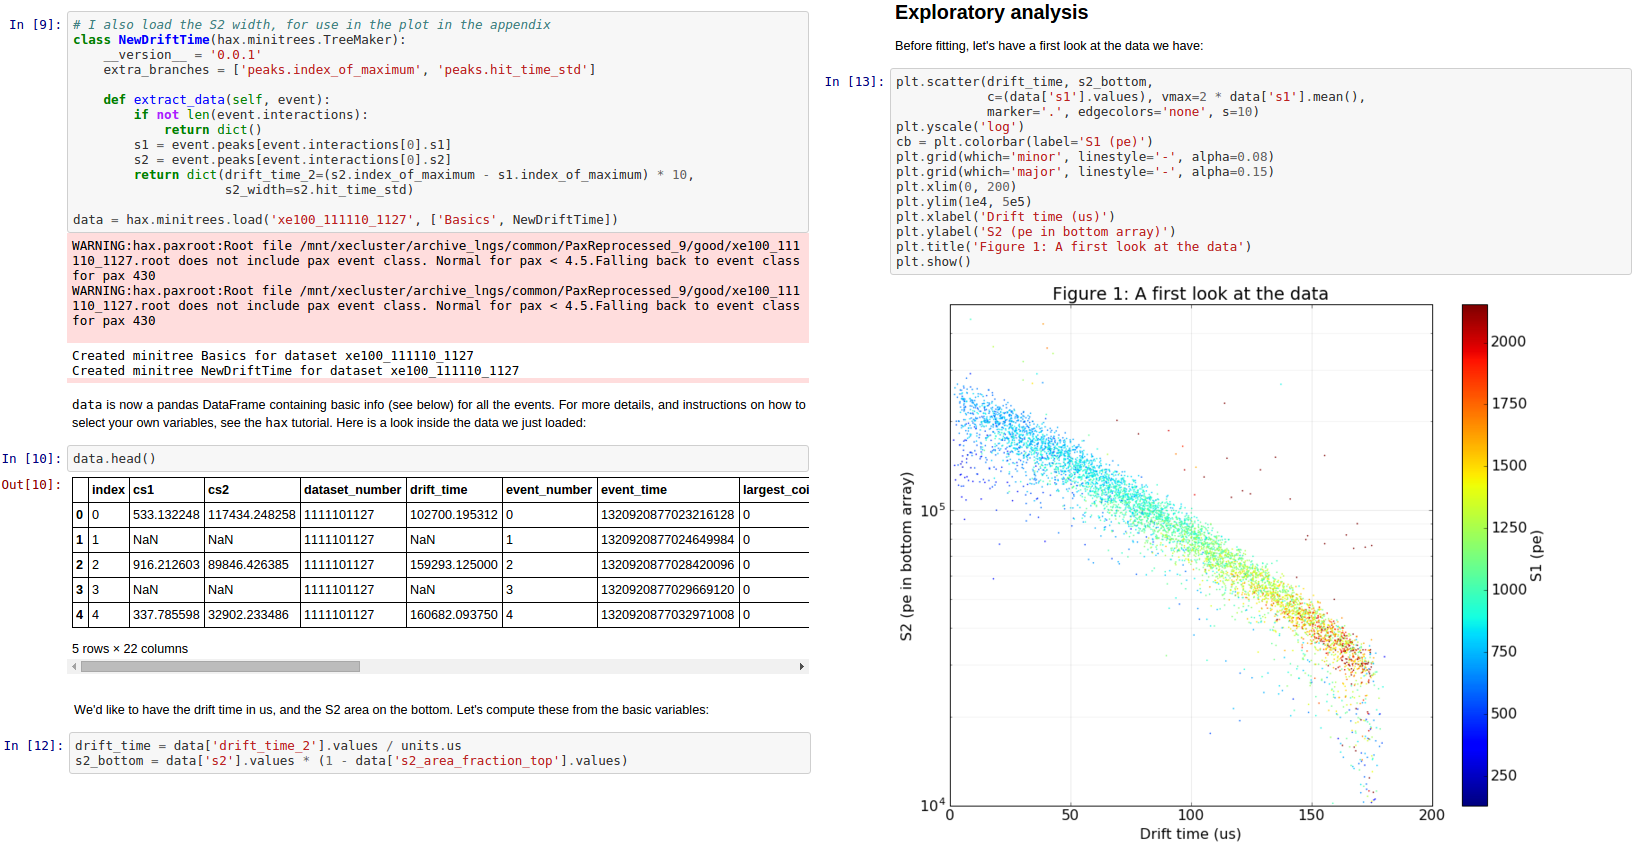
\includegraphics[width=1.05\linewidth]{./graphics/hax_in_action.png}
\caption{HAX in action: IPython notebook demonstrating how to: (1) create a mini-tree containing selection of variables in the dataset; (2) load the data in a pandas DataFrame; (3) perform exploratory visual analysis with matplotlib }
\label{fig:hax_in_action}
\end{center}
\end{figure}
\end{landscape}

% \section{Conclusions and future work} % <-- or ``Summary and Outlook''
% \lipsum[1-2]
% maybe not, CHEP papers usually ``keep it short'' without repetitions at intro and conclusions


\section{Acknowledgments}
This work was supported by a pathfinder project in collaboration with the Netherlands eScience Center.
The authors would like to thank the XENON, PyROOT, and rootpy community for their valuable contribution and impact on this work.
% This work was supported by pathfinder project... 
%  This work is in part funded by
% the research programme of the Netherlands eScience Center.
\section*{References}
\bibliographystyle{iopart-num}
\bibliography{chep2016_remenska}
% \begin{thebibliography}{9}
% \bibitem{iopartnum} IOP Publishing is to grateful Mark A Caprio, Center for 
% Theoretical Physics, Yale University, for permission to include the {\tt 
% iopart-num} \BibTeX package (version 2.0, December 21, 2006) with  this 
% documentation. Updates and new releases of {\tt iopart-num} can be found on 
% \verb"www.ctan.org" (CTAN). 
% \end{thebibliography}

\end{document}


